\documentclass[tikz,border=10pt]{standalone}
\usepackage{amsmath, amssymb}
\usetikzlibrary{shapes.geometric, arrows.meta, positioning, fit, calc, backgrounds}

\begin{document}
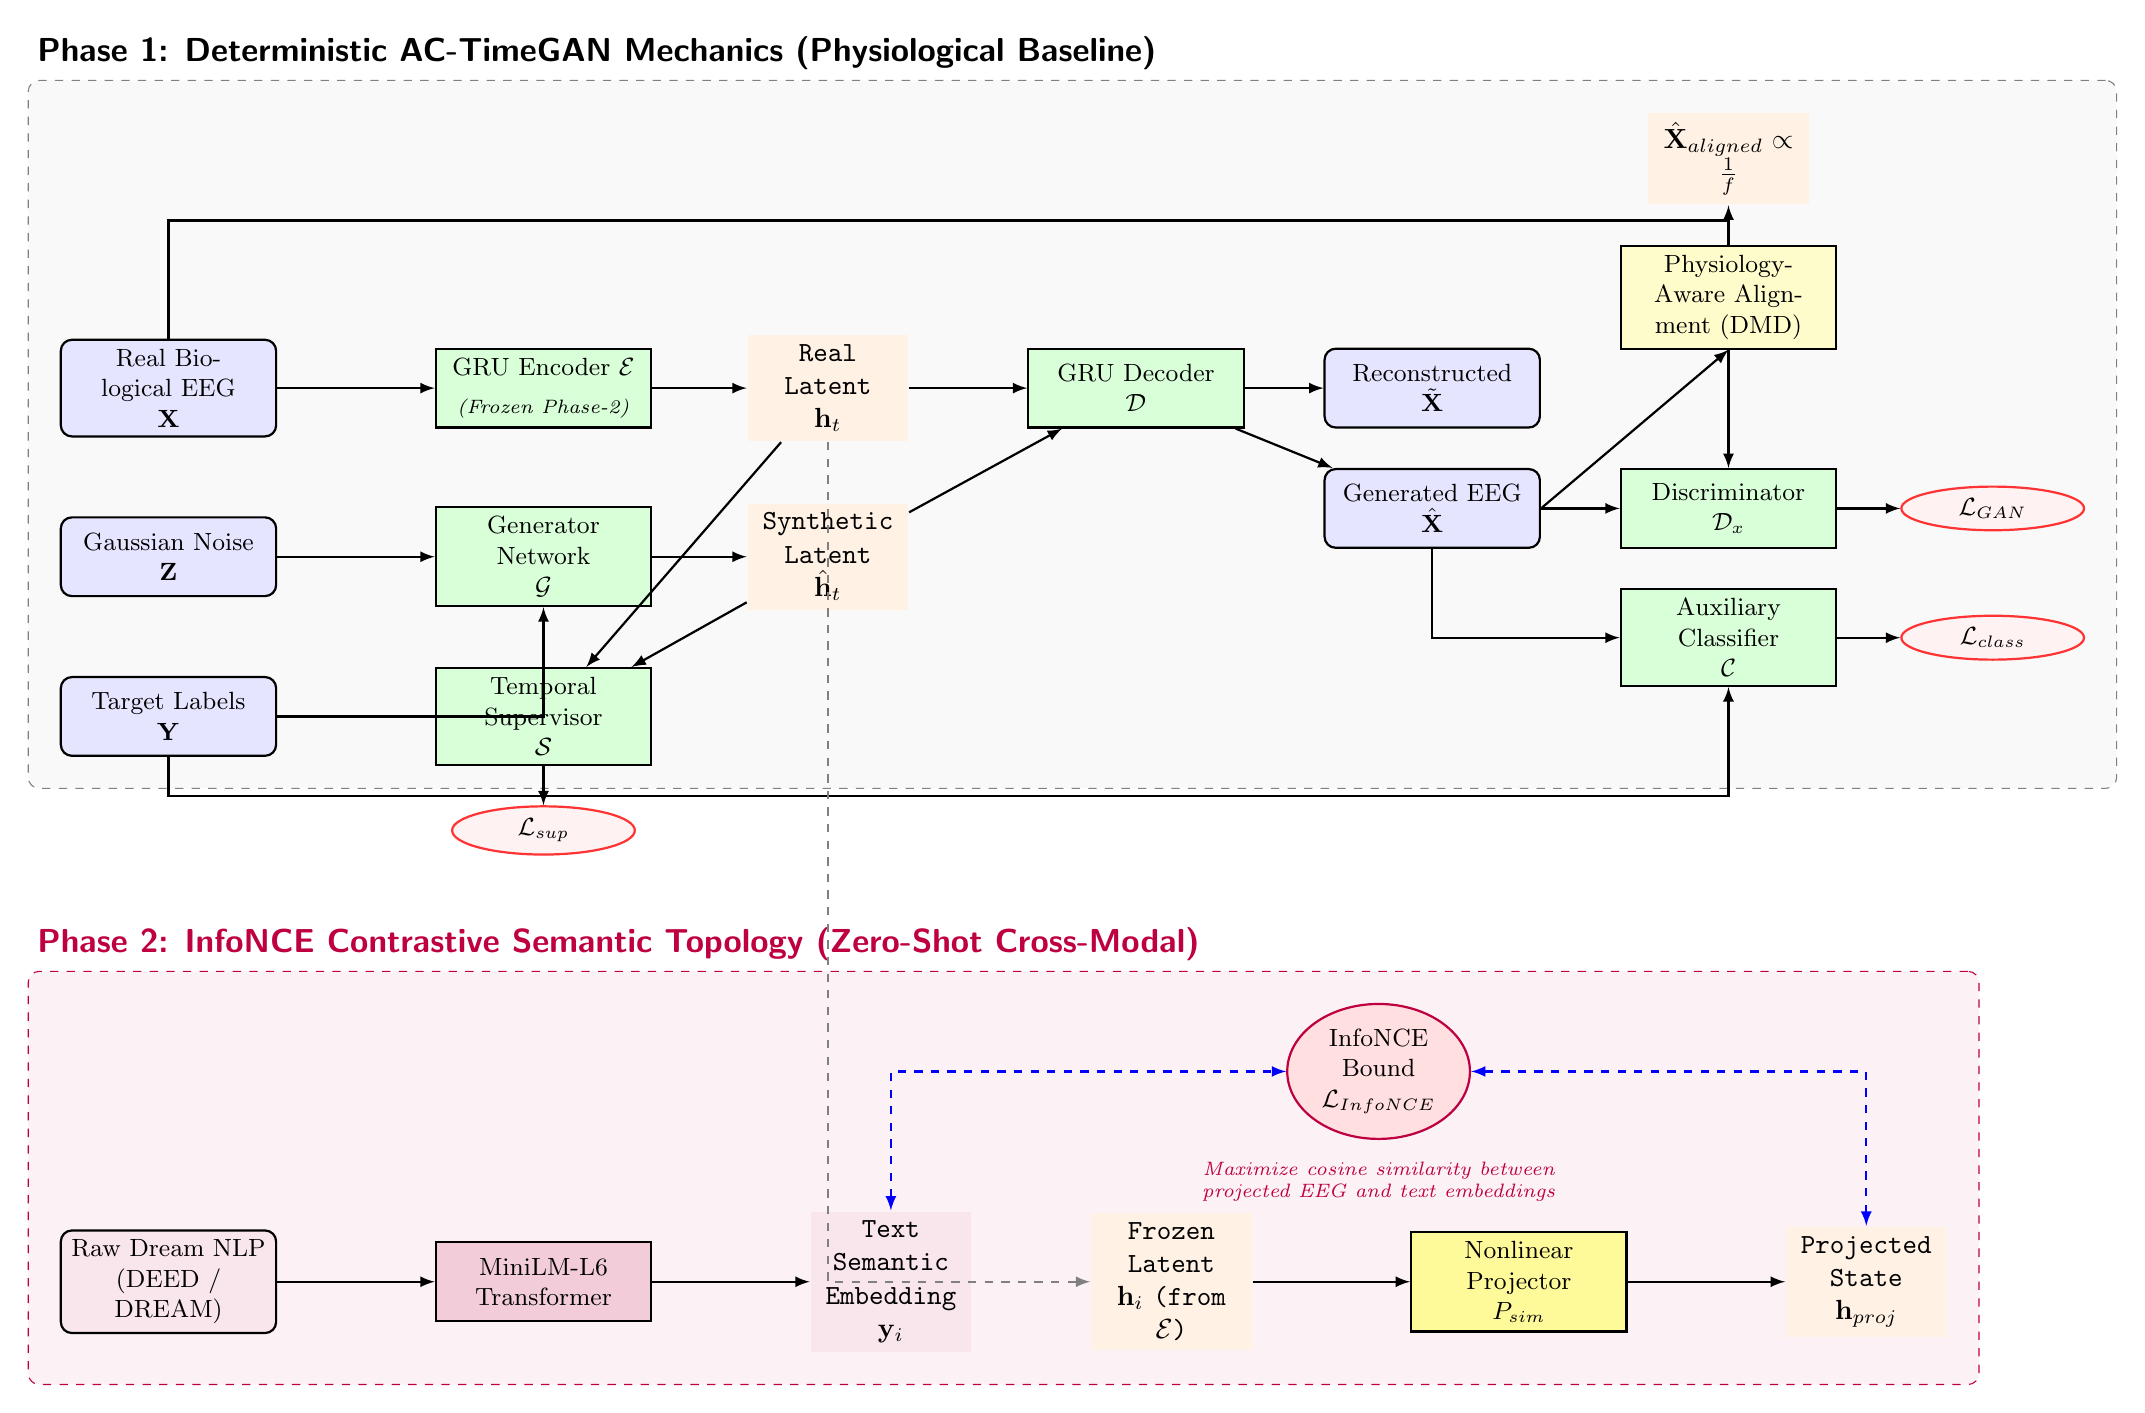
\begin{tikzpicture}[
    node distance=1.5cm and 2cm,
    font=\small,
    thick,
    % Core Blocks
    data/.style={rectangle, draw=black, fill=blue!10, text width=2.5cm, align=center, rounded corners, minimum height=1cm},
    network/.style={rectangle, draw=black, fill=green!15, text width=2.5cm, align=center, minimum height=1cm},
    loss/.style={ellipse, draw=red!80, fill=red!5, text width=1.5cm, align=center, inner sep=2pt},
    label/.style={rectangle, draw=none, fill=none, text width=2cm, align=center, font=\bfseries},
    math/.style={rectangle, draw=none, fill=orange!10, text width=1.8cm, align=center, font=\ttfamily},
    % Arrow styles
    forward/.style={->, >=latex, thick},
    backprop/.style={->, >=latex, dashed, red, thick},
    sync/.style={<->, >=latex, dashed, thick, blue}
]

    % =========================================================
    % PHASE 1: DETERMINISTIC AC-TIMEGAN MECHANICS
    % =========================================================
    
    % Data & Noise Inputs
    \node[data] (realx) {Real Biological EEG\\ $\mathbf{X}$};
    \node[data, below=1cm of realx] (noise) {Gaussian Noise\\ $\mathbf{Z}$};
    \node[data, below=1cm of noise] (labels) {Target Labels\\ $\mathbf{Y}$};
    
    % Embedders & Generators
    \node[network, right=of realx] (embedder) {GRU Encoder $\mathcal{E}$\\ \vspace{0.1cm}\scriptsize\textit{(Frozen Phase-2)}};
    \node[network, right=of noise] (generator) {Generator Network\\ $\mathcal{G}$};
    \node[network, right=of labels] (supervisor) {Temporal Supervisor\\ $\mathcal{S}$};
    
    % Connections from Data
    \draw[forward] (realx) -- (embedder);
    \draw[forward] (noise) -- (generator);
    \draw[forward] (labels) -| (generator);
    
    % Latent States
    \node[math, right=1.2cm of embedder] (latenth) {Real Latent\\ $\mathbf{h}_t$};
    \node[math, right=1.2cm of generator] (synthh) {Synthetic Latent\\ $\hat{\mathbf{h}}_t$};
    
    \draw[forward] (embedder) -- (latenth);
    \draw[forward] (generator) -- (synthh);
    
    % Supervisor and Generation Dynamics
    \draw[forward] (latenth) -- (supervisor) node[midway, left] {};
    \draw[forward] (synthh) -- (supervisor) node[midway, left] {};
    \node[loss, below=0.5cm of supervisor] (loss_sup) {$\mathcal{L}_{sup}$};
    \draw[forward] (supervisor) -- (loss_sup);
    
    % Decoder block
    \node[network, right=1.5cm of latenth] (decoder) {GRU Decoder\\ $\mathcal{D}$};
    \draw[forward] (latenth) -- (decoder);
    \draw[forward] (synthh) -- (decoder);
    
    % Reconstructed sequences
    \node[data, right=1cm of decoder] (reconx) {Reconstructed\\ $\tilde{\mathbf{X}}$};
    \node[data, below=0.5cm of reconx] (synthx) {Generated EEG\\ $\hat{\mathbf{X}}$};
    \draw[forward] (decoder) -- (reconx);
    \draw[forward] (decoder) -- (synthx);
    
    % Discriminator and Auxiliary Classifier
    \node[network, right=1cm of synthx] (discriminator) {Discriminator\\ $\mathcal{D}_x$};
    \node[network, below=0.5cm of discriminator] (classifier) {Auxiliary Classifier\\ $\mathcal{C}$};
    
    \draw[forward] (synthx) -- (discriminator);
    \draw[forward] (synthx) |- (classifier);
    
    \draw[forward] (realx.north) -- ++(0,1.5) -| (discriminator.north);
    \draw[forward] (labels.south) -- ++(0,-0.5) -| (classifier.south);
    
    \node[loss, right=0.8cm of discriminator] (loss_gan) {$\mathcal{L}_{GAN}$};
    \node[loss, right=0.8cm of classifier] (loss_class) {$\mathcal{L}_{class}$};
    \draw[forward] (discriminator) -- (loss_gan);
    \draw[forward] (classifier) -- (loss_class);
    
    % PAA Algorithm Block
    \node[network, fill=yellow!20, above=1.5cm of discriminator] (paa) {Physiology-Aware Alignment (DMD)};
    \draw[forward] (synthx.east) -- (paa.south);
    \node[math, above=0.5cm of paa] (paa_math) {$\hat{\mathbf{X}}_{aligned} \propto \frac{1}{f}$};
    \draw[forward] (paa) -- (paa_math);
    
    % Phase 1 Bounds
    \begin{scope}[on background layer]
        \node[fit=(realx)(noise)(labels)(embedder)(generator)(decoder)(discriminator)(classifier)(paa)(paa_math)(loss_gan)(loss_class), fill=gray!5, rounded corners, draw=gray, dashed, inner sep=0.4cm] (phase1box) {};
        \node[above right, font=\large\bfseries\sffamily, color=black] at (phase1box.north west) {Phase 1: Deterministic AC-TimeGAN Mechanics (Physiological Baseline)};
    \end{scope}

    % =========================================================
    % PHASE 2: SEMANTIC ALIGNMENT (INFONCE)
    % =========================================================
    
    % Semantic Inputs
    \node[data, below=6.0cm of labels, fill=purple!10] (text_input) {Raw Dream NLP\\ (DEED / DREAM)};
    \node[network, right=of text_input, fill=purple!20] (transformer) {MiniLM-L6\\ Transformer};
    \node[math, right=of transformer, fill=purple!10] (y_anchor) {Text Semantic\\ Embedding $\mathbf{y}_i$};
    
    \draw[forward] (text_input) -- (transformer);
    \draw[forward] (transformer) -- (y_anchor);
    
    % Projection Head from locked Latents
    \node[math, right=1.5cm of y_anchor, fill=orange!10] (frozen_h) {Frozen Latent\\ $\mathbf{h}_i$  (from $\mathcal{E}$)};
    \node[network, right=of frozen_h, fill=yellow!40] (projection) {Nonlinear Projector\\ $P_{sim}$};
    \node[math, right=of projection, fill=orange!10] (h_proj) {Projected State\\ $\mathbf{h}_{proj}$};
    
    \draw[forward, dashed, color=gray] (latenth.south) |- (frozen_h.west);
    \draw[forward] (frozen_h) -- (projection);
    \draw[forward] (projection) -- (h_proj);
    
    % InfoNCE Space
    \path (y_anchor) -- (h_proj) coordinate[midway] (mid_proj);
    \node[loss, fill=pink!50, draw=purple, above=1.8cm of mid_proj] (infonce) {InfoNCE Bound\\ $\mathcal{L}_{InfoNCE}$};
    \node[font=\scriptsize\itshape, text=purple, align=center, below=0.15cm of infonce] {Maximize cosine similarity between\\ projected EEG and text embeddings};
    \draw[sync] (y_anchor.north) |- (infonce.west);
    \draw[sync] (h_proj.north) |- (infonce.east);
    
    % Phase 2 Bounds
    \begin{scope}[on background layer]
        \node[fit=(text_input)(transformer)(y_anchor)(frozen_h)(projection)(h_proj)(infonce), fill=purple!5, rounded corners, draw=purple, dashed, inner sep=0.4cm] (phase2box) {};
        \node[above right, font=\large\bfseries\sffamily, color=purple] at (phase2box.north west) {Phase 2: InfoNCE Contrastive Semantic Topology (Zero-Shot Cross-Modal)};
    \end{scope}

\end{tikzpicture}
\end{document}
